\section{Start-up and shut-down procedures for agreed plant section}
The start-up and shutdown procedures for the agreed plant section were elaborated based on the recommendations proposed by \textcite{bp_international_safe_2006}. The guiding principles are presented, followed by the detailed start-up and shut-down procedures. Calculations for the time allocated to various steps can be found in \Cref{app:samplecal}.

It should be noted that extra vessels to temporally store off-specification material produced during start-up and shutdown are available in the plant subsection. Moreover, any waste material from start-up and shutdown is sent the on-site waste treatment plant. Liquid wastes first undergo adsorption using activated carbon, followed by anaerobic membrane treatment. Prior to this, waste streams with high nitric acid content willGaseous wastes are disposed of via incineration.Further details on waste disposal can be found in \Cref{sec:waste}.

\subsection{Start-up standard operating procedure}

\paragraph{Preliminary preparations}
Prior to operation, all units should the inspected to ensure all maintenance and shutdown work have been completed and that the unit is fit for operation. The inspection step also entails the removal of any foreign material in the plant section. Those typically include scaffolding and tools which must be removed from the operating area as they can cause obstructions during emergencies. It must also be verified that no foreign substance has entered the units during shutdown, to avoid possible explosions. Checks for fouling are also performed. The shutdown blinds are then removed and replaced by running blinds. A check list of blinds needs to be established to make sure no blind is overlooked as this may cause damage to pipes and equipment.



\paragraph{Auxiliary equipment and utilities start-up}

Electricity units are the first utility to be checked and tested for moisture accumulation and potential defects. Critical instruments and valves, alarms, automatic shutdown devices and other safety features are then checked and activated as soon aspossible.
The opening of the steam system takes place gradually to prevent thermal and mechanical shocks. The cooling water system is also brought to operation by opening the relevant valves. The electrical heaters are tested and prepared to ensure they can deliver the required heating duty. The motor of the fan is started to verify it can deliver the gas flow required. 

\paragraph{Elimination of air and leak prevention}
Since the system is composed of highly flammable chemicals, it is crucial to ensure oxidisers, such as oxygen, are absent from the plant section. To do so, air must be purged before the introduction of the reagents. Nitrogen purging is favoured over steam purging and other techniques due to the presence of the catalyst packed bed. Purging of the system also discloses plugged drains and vents. It is assumed a nitrogen feed line is available in the plant subsection. 
The purge gas is then pressurised to be used in tightness testing to check for leaks. The test is performed at 3.5 barg or 0.7 barg blow the lower relief valve set point, which ever is lower. Once all vents have been closed, inspection for leaks at joints, flanges, heater plugs, vents and drains is carried out. If tightening of the bolts is insufficient to fix a leak, the unit must be depressurised, fixed and repurged.

\paragraph{Initiation of on-stream units}
Once a unit in air and leak free, it can be brought onstream by adjusting the pressures, temperatures, flowrates and levels until the unit reaches its normal operating conditions. To avoid thermal or mechanical shocks, changes in temperature, pressure and flow should be gradual and uniform. Overpressure must be avoided by ensuring there is no blockage in outlet lines.


\subsubsection{Start-up control sequence}
\begin{figure}[h]
    \centering
    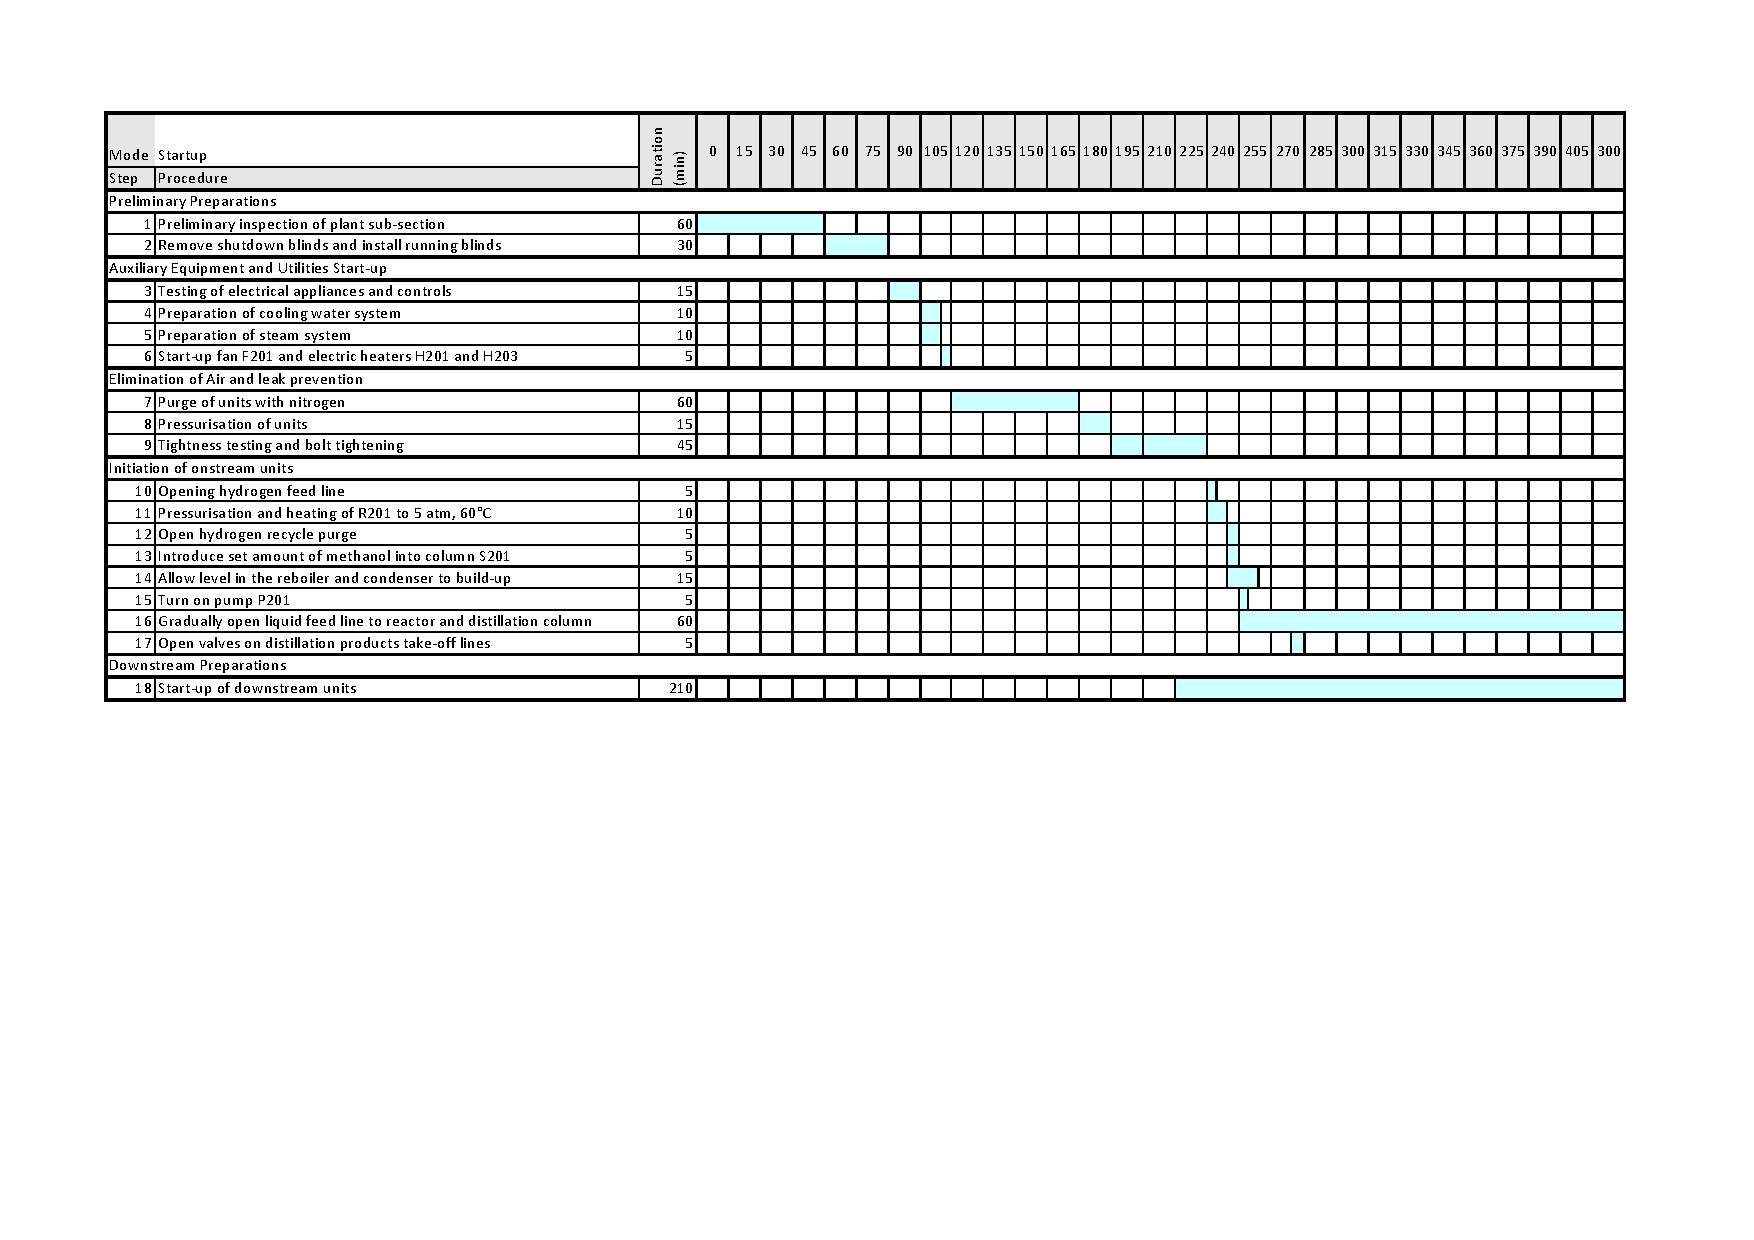
\includegraphics[clip, trim= 1cm 8cm 1cm 1.5cm, width=\linewidth]{chapters/4-operation-control/4-Figures/Shart-up.pdf}
    \caption{Gantt chart of shart-up SOP}
    \label{fig:startup}
\end{figure}



\begin{itemize}
    \item Step 4: To prepare the cooling water system, valves FCV-201 and FCV-204 have to be opened. It is assumed that equipment outside this section pump the cooling water to the plant.
    \item Step 5: The steam system is started by opening valves FCV-207 and SOV-205.
    \item Step 6: The motor of the fan F201 is started and the electric heaters H201 and H203 are turned on. 
    \item Step 7: To purge the units with nitrogen, the drain and vent valves (SOV-203, SOV-204, SOV-206, SOV-207 SOV-208, SOV-209), and the valves connecting the reactor to the distillation column  (FCV-203, PCV-201) are open. 
    \item Step 8: To pressurise the units, valves drain and vent valves (SOV-203, SOV-204, SOV-206, SOV-207 SOV-208, SOV-209), the valves connecting the reactor to the distillation column (FCV-203, PCV-201) and the outlet valves (FCV-206, FCV-208, FCV-205) are closed. 
    \item Step 10: Valves SOV-202, PCV-202, V201, V202 and V203 are gradually opened to begin the flow of hydrogen to the plant and pressurise reactor R201.
    \item Step 12: The hydrogen recycle purge is open via valve FCV-202.
    \item Step 13-14: With valves SOV-206, SOV-209, SOV-208, FCV-205, FCV-206 and FCV-208 closed, methanol is introduced into the column S203.
    \item Step 15-16: The liquid feed stream lie is activated by opening the valves SOV-201, V206 and V207.
    \item Step 17: The flow control valve FCV-205, FCV-206 and FCV-208 are open to send the outlets to the downstream units.
\end{itemize}


\subsection{Shutdown standard operating procedure}

\paragraph{Cooling and depressurising units}
The removal and dissipation of stored energy (heat and pressure) from process units is performed first in order to prevent fires, explosions or other hazardous events from occurring in later stages. Sources of heating are turned off and allowed to cool to ambient temperatures, and feed streams are gradually reduced in order to prevent sensitive process equipment (centrifugal pumps and transmitters) from being damaged by sudden loss of fluid. Cooling water is kept flowing in order to dissipate thermal energy from the process units. Product lines from the distillation tower are gradually reduced in accordance with the reduction in feed rate, and the hydrogen in the reactor is purged to a gas collection system.

\paragraph{Pumping out of process fluids}
Process liquids remaining in each unit are drained, and reciprocating pumps may be installed and used when the hydrostatic pressure in the unit reduces. Inert gas such as nitrogen should be pumped into units with mostly liquid holdup in order to prevent a vacuum from developing. Vapours at atmospheric pressures are also purged from the system using inert gas to a gas collection system.

\paragraph{Purging residual materials and water disposal}
A further purging step is required to ensure good removal of residual process fluids and hydrocarbons in the process units. While steam is a common purging gas, it is undesirable in our sub-section due to the presence of a packed reactor and column. The condensation of water on the packings would affect porosity in the packed beds, and the freezing of water droplets may damage the catalyst in the reactor. Thus an inert gas like nitrogen is preferred. The nitrogen purge should flow continually from the first unit until the end of the process line to ensure no area in the sub-section is bypassed. Each unit should be tested for hydrocarbon content using gas indicators, and when enough purge gas has flowed to reduce the hydrocarbon content below 1\%, the vents and drain pipes should be closed to conserve purge gas. 

When the cooling water supply is shut off, care must be taken to ensure that the trace amounts of water remaining in the network do not freeze, as that could prevent shutoff valves closing properly, or damage mechanical equipment. Weep holes must be installed in the condenser baffles, and the system should be blown out with hot gas.

\paragraph{Blinding and opening}
Shutdown blinds are usually installed on utility lines and process lines for equipment that requires personnel access. These need to be in place to prevent unwanted fluids flowing through the plant when undergoing maintenance. Blinds should exchanged slowly with extreme care, so that any spillages can be contained more easily. 

\paragraph{Inspection for entering}
The internals of the reactor and packed column in our sub-section would require regular inspections, particularly to check for structural integrity of the packing and catalyst deactivation. These units need to be physically disconnected from the rest of the plant during shutdown by removing isolation valves and blanking open ends. Prior to entry, the environment in the unit must be tested for normal oxygen levels and safe levels of toxic or combustible gases. The gas vents must be open. 


\subsubsection{Shutdown control sequence}
\begin{figure}[h]
    \centering
    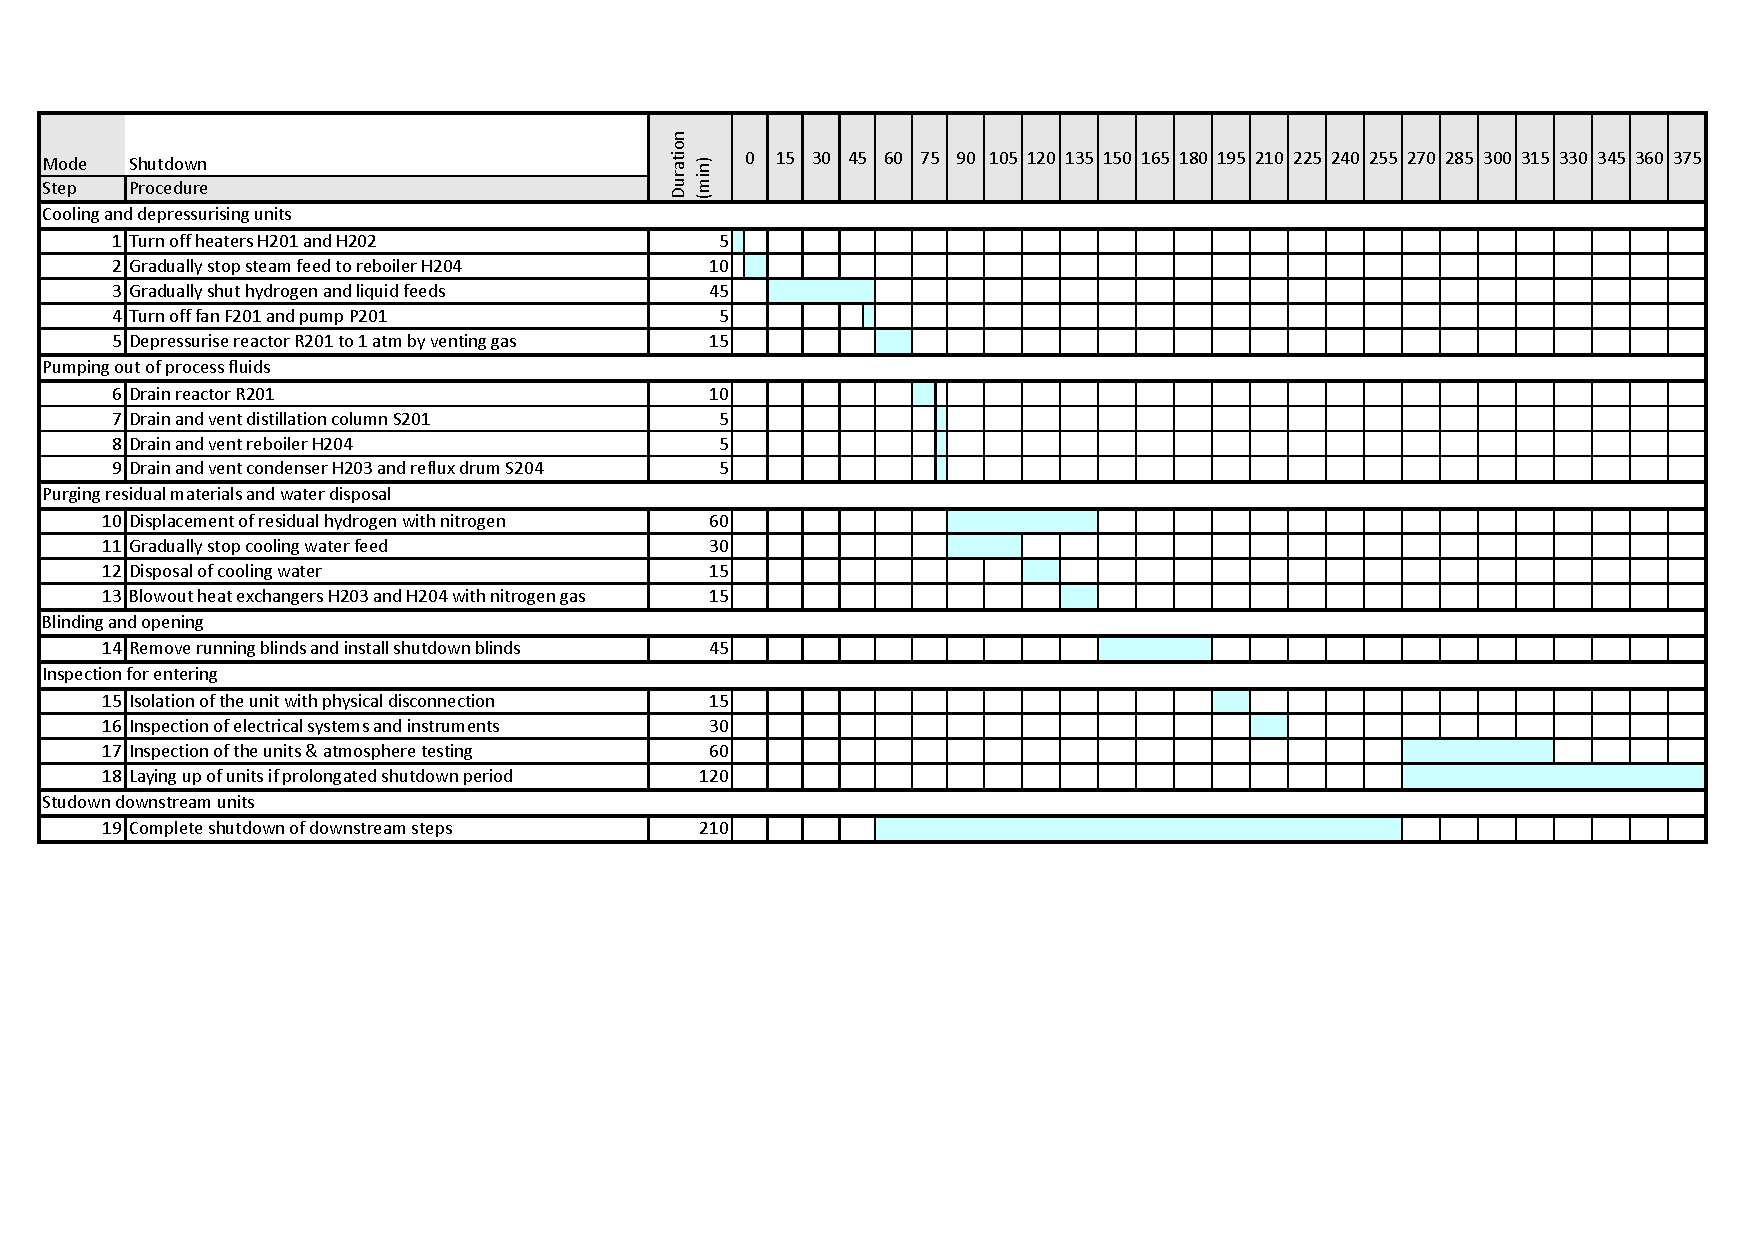
\includegraphics[clip, trim= 0.5cm 6cm 0.5cm 1cm, width=\linewidth]{chapters/4-operation-control/4-Figures/Shutdown.pdf}
    \caption{Gantt chart of shutdown SOP}
    \label{fig:shutdown}
\end{figure}


\begin{itemize}
    \item Step 2: Stop the steam feed to reboiler using FCV-207. 
    \item Step 3: The hydrogen and liquid feeds are gradually stopped using V206 and V202, and are fully shut off by closing SOV-201, SOV-202. Care must be taken to turn the pump off before it runs dry. 
    \item Step 5: The reactor is vented by keeping SOV-204, the vapour outlet port and FCV-202 open.
    \item Step 6-9: Drain and vent valves (SOV-203, SOV-206, SOV-207, SOV-208, SOV-209) are opened to remove process fluids from the vessels.
    \item Step 10: The drain, vent and flow control valves across the sub-section should manually be kept open to allow nitrogen to flow and remove any remaining process fluids. Once each unit is safe, the drains and vents in that unit are closed to conserve purge gas. 
    \item Step 11-13: Cooling water is gradually turned off using FCV-201 and FCV-204. Hot nitrogen is then blown through to completely dry these lines.
    \item Step 15-18: The units should only be physically disconnected from the plant when downstream units have been drained and purged, to avoid back-flow and spillage of process fluids from the open pipe ends.
\end{itemize}